	Como interfaz entre la FPGA y la PC se utilizó kit de de desarrollo CY3684 FX2LP EZ-USB Development Kit de Cypress Semiconductor,la que se observa en la Figura \ref{cy3684}. Esta placa posee como núcleo el controlador USB CY7C68013A, circuito integrado que posee todas las herramientas necesarias para realizar la interfaz, como así también un buen número de periféricos que permiten al desarrollador realizar pruebas y depuración.\\
	
	\begin{figure}
		\centering
		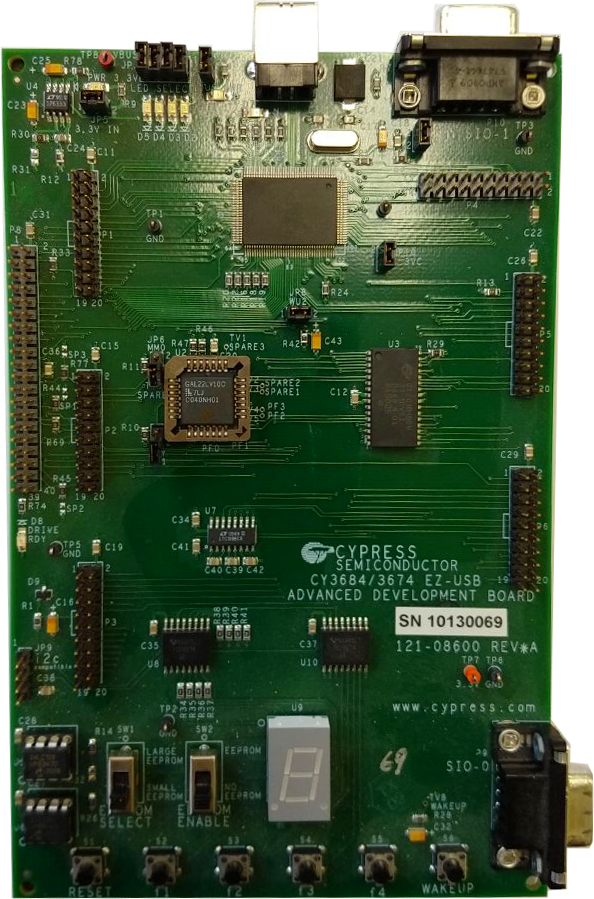
\includegraphics[width=0.4\textwidth]{32cypressboard}
		\caption{Circuito impreso principal del kit de desarrollo CY3684 FX2LP EZ-USB}
		\label{cy3684}
	\end{figure}
	
	Entre estas, se destacan 6 pulsadores, de los cuales cuatro se utilizan para proposito general, uno para reestablecer los valores por defecto de la placa y uno para enviar señales de suspensión y reestablecimiento del programa actualmente cargado en el microcontrolador, lo que coloca al sistema en modo bajo consumo de energía. A su vez, posee dos memorias EEPROM que sirven para cargar firmware y archivos de configuración del sistema, un display de 8 segmentos, 4 leds de multiple propósito, dos puertos UART, una salida de pines compatible con puertos ATA y 6 puertos de 20 pines que se utilizan para la conexión hacia el chip núcleo. Como soporte para el firmware, posee también un bloque con \SI{64}{\kilo\byte} de memoria SRAM.\\
	
	Se selecciona este controlador como interfaz con el objetivo de utilizar la menor cantidad de los recursos configurables de la FPGA, de forma tal que estos queden disponibles para el desarrollo de sistemas científicos complejos que sean necesarios a posteriori.\\
	